\chapter{Modellbildung}
\label{chap:modellbildung}
In unserem Model wird das Nicken und Rollen vernachlässigt, weil wir uns das Fahrverhalten auf einer vertikalen, ebenen Fläche anschauen wollen. 
Die abzufahrende Soll-Strecke soll bestmöglich abgefahren werden. Mittels Regler wird die Differenz der Soll- und der Ist-Werte errechnet. Daraus werden Steuersignale an die Aktuatoren weitergeleitet, die den Kurs oder die Geschwindigkeit korrigieren. Dazu ist es notwendig, die tatsächlichen Werte des Fahrzeuges (wie etwa die Geschwindigkeit oder die Position) zu ermitteln.  

\section{Verwendete Koordinatensysteme}
Zur Beschreibung der Fahrzeugbewegung stehen verschiedene Koordinatensysteme zur Verfügung. Im Folgenden werden die drei Koordinatensysteme vorgestellt: 
\begin{itemize}
\item weltfestes Koordinatensystem $F_w ={x_w,y_w,0}$ 
\item fahrzeugfestes Koordinatensystem auf Höhe des Fahrzeugschwerpunkts $F_f ={P_f,x_f,y_f}$
\item Straßenkoordinatensystem $F_r ={P_r,s_r,d_r}$ 
\end{itemize}
Die einfachste Darstellung der Fahrzeugbewegung geschieht im weltfesten Koordinatensystem $F_w$, in dem die absolute Position des Fahrzeugs abzulesen ist. Ursprung und Ausrichtung sind an einen Ort gebunden und werden durch die Koordinaten $[x_w,yw]$ beschrieben. Das fahrzeugfeste Koordinatensystem $F_f$ hat den Ursprung im Punkt $P_f$, dem Fahrzeugschwerpunkt $s_1$. Es wird durch die Koordinaten $[x_f,y_f]$ beschrieben und ist so orientiert, dass die $x_f$-Achse jederzeit der Fahrzeuglängsachse entspricht und nach vorne gerichtet ist. Die $y_f$-Achse steht entsprechend senkrecht zur Fahrzeuglängsachse und zeigt nach links. Es bewegt sich also mit dem Fahrzeug mit, anders als das weltfeste Koordinatensystem. 
Zum Fahren entlang einer Fahrspur reicht die fahrzeugfeste Position aus, um relativ zur Fahrspur und anderen Verkehrsteilnehmern navigieren zu können. Dazu eignet sich die Darstellung im Straßenkoordinatensystem $F_r$. Mathematisch lässt sich das durch die sog. Frenet-Koordinaten $[s_r,d_r]$ beschreiben. Diese werden durch die Bogenlänge $s_r$ und den Abstand zur Fahrspur $d_r$ beschrieben. Der Tangentenvektort($s_r$)ist dabei immer tangential zum Pfad der Straße ausgerichtet und der Normalenvektor n($s_r$) steht senkrecht dazu und zeigt auf den Referenzpunkt des Fahrzeugs (Fahrzeugschwerpunkt $P_f$).


\section{Bewegungsgleichungen}
Newtons allgemeine Form der Bewegungsgleichung ist
\begin{equation}
  m\cdot a = \sum F  
\end{equation}
Die Massenträgheit ist die Masse multipliziert mit der Beschleunigung und ist auch die Summe aller, von außen wirkenden, Kräfte in dem System.
Bei dem System zum autonomen Fahren handelt es sich dabei um Folgende Kräfte:
\begin{itemize}
\item Zugkraft $F_a = \frac{M}{r} $
\item Straßenwiderstand $F_rr = m\cdot g\cdot C$
\item Luftwiderstand $F_aero = \frac{1}{2}\rho C A V^{2}$
\end{itemize}
Dabei ist $M$ das Drehmoment des Motors, $r$ der Radius eines Rades, $\rho$ die Luftdichte[kg/$m^{3}$], $A$ die Fahrzeugoberfläche orthogonal zur Bewegungsrichtung, $C$ der Koeffizient und $v$ die Geschwindigkeit (Der Luftwiderstand nimmt also quadratisch mit der Geschwindigkeit zu).\\
Setzt man das in die Bewegungsgleichung ein, erhält man
\begin{equation}
  m\cdot a = F_a -  F_rr - F_aero 
\end{equation}
\begin{equation}
  m\cdot a = F_a -  m\cdot g\cdot C - \frac{1}{2}\rho C A V^{2} 
\end{equation}
Teilt man auf beiden Seiten Der Gleichung durch $m$, erhält man die Beschleunigung des Fahrzeugs:
\begin{equation}
  a = \frac{F_a}{m} -  \frac{m\cdot g\cdot C}{m} - \frac{\frac{1}{2}\rho C A V^{2}}{m} 
\end{equation}
\begin{equation}
  a = \frac{F_a}{m} -  g\cdot C - \frac{\frac{1}{2}\rho C A V^{2}}{m} 
\end{equation}
Die Ableitung einer Strecke nach der Zeit ergibt die Geschwindigkeit. Die Ableitung einer Geschwindigkeit nach der Zeit ergibt die Beschleunigung. Sei $x$ die Strecke des Fahrzeugs, dann ist $\dot{x}$ die Geschwindigkeit und $\ddot{x}$ die Beschleunigung.
Damit können wir die Variablen aus der Gleichung ersetzten und erhalten:
\begin{equation}
 \ddot{x} = \frac{F_a}{m} -  g\cdot C - \frac{\frac{1}{2}\rho C A \dot{x}^{2}}{m} 
\end{equation}
So lässt sich leicht erkennen, dass es sich bei dieser Gleichung um eine Differentialgleichung (DGL) zweiter Ordnung handelt. Daraus machen wir jetzt im folgendem Schritt zwei DGL, jeweils erster Ordnung:
\begin{equation}
 x_1=v 
\end{equation}
\begin{equation}
  x_2=\dot{v} 
\end{equation}
Bestimmen von Zustandsvariablen (die Variablen spannen einen Raum im zweidimensionalen Raum, weshalb es so viele Zustandsvariablen gibt, wie es Ordnungen im System gibt):\\
1. Zustandsvariablen miteinander verknüpfen:
\begin{equation}
  \dot{x_1} = x_2 
\end{equation}
2. Einsetzen:
\begin{equation}
  \dot{x_2} = \frac{F_a}{m} -  g\cdot C - \frac{\frac{1}{2}\rho C A {x1}^{2}}{m} 
\end{equation}



\section{Differentialantrieb} 
Wir modellieren das Fahrverhalten anhand eines Fahrzeuges mit zwei Antriebsrädern und einem Stützrad. Gelenkt wird nur über die unterschiedlichen Geschwindigkeiten der einzeln ansteuerbaren Antriebsräder. Wir benutzen zwei Koordinatensysteme, ein Fahrzeugfestes, dessen Ursprung im Fahrzeugmittelpunkt liegt und dessen x-Achse in Richtung des Roboterfrontteils zeigt. die Pose p gibt Auskunft über Position im Weltfesten Koordinatensystem und Winkel zwischen Fahrzeug- und Weltfesten x-Achse.  
\begin{figure}[htb]
  \centering  
  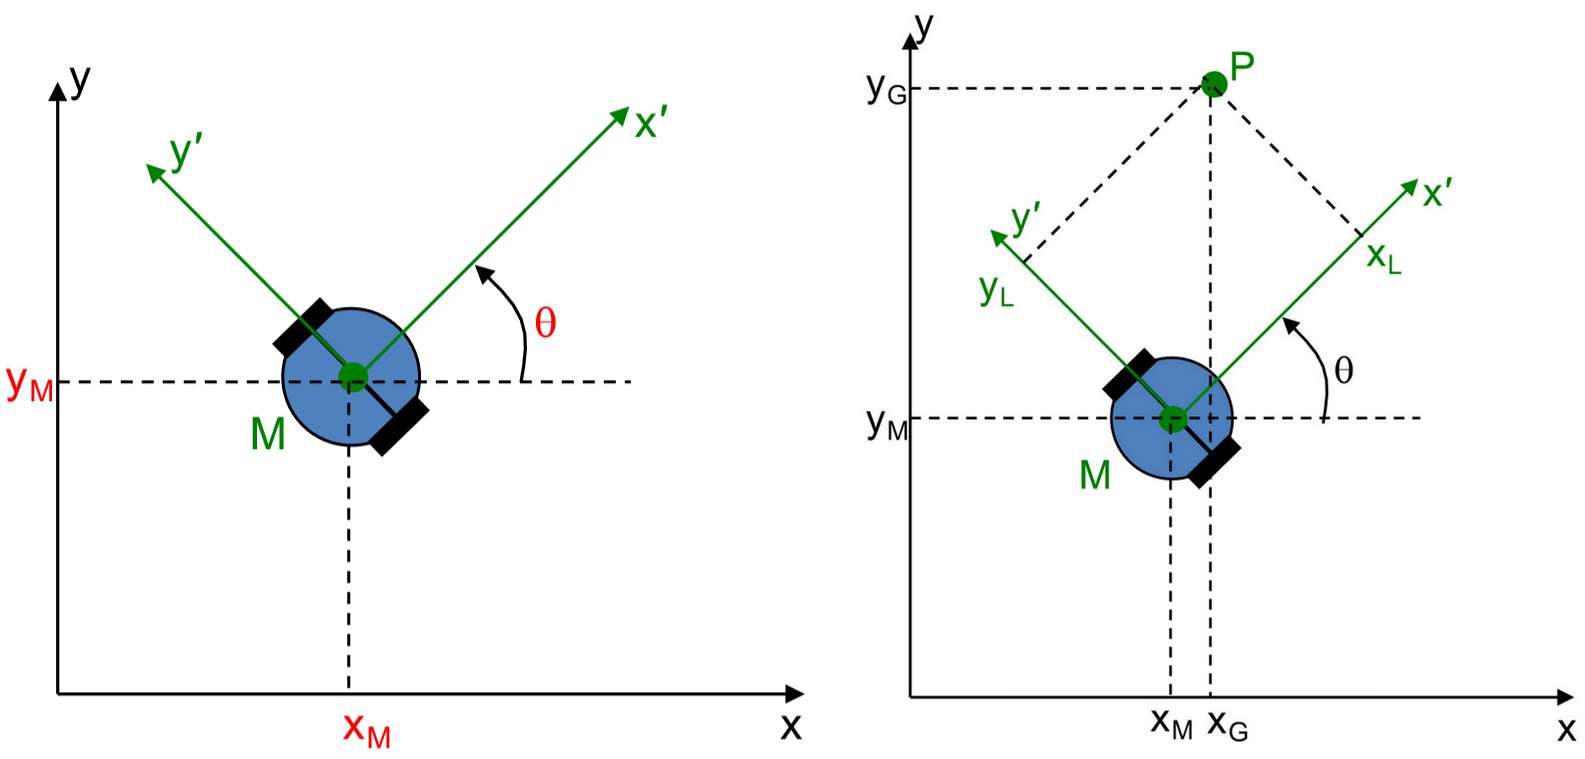
\includegraphics[scale=1]{img/einfachesModell_1.png}
  \caption{Weltfestes- und Fahrzeugfestes Koordinatensystem\cite{robot}}
  \label{fig:Weltfestes- und Fahrzeugfestes Koordinatensystem}
\end{figure}
\begin{equation}
p =
\begin{bmatrix}
x_{weltfest}\\
y_{weltfest}\\
\Theta \\
\end{bmatrix}
\end{equation}
Ein Punkt im Fahrzeugfesten Koordinatensystem F sei: 
\begin{equation}
p_{F} =
\begin{bmatrix}
x_{F}\\
y_{F}\\
\end{bmatrix}
\end{equation}
Der selbe Punkt ist im Weltfesten Koordinatensystem definiert als: 
\begin{equation}
p_{W} =
\begin{bmatrix}
x_{W}\\
y_{W}\\
\end{bmatrix}
\end{equation}
Mit Hilfe der so genannten Rotationsmatrix 
\begin{equation}
R(\Theta) = 
\begin{bmatrix}
cos \Theta & -sin \Theta\\
sin \Theta & cos \Theta\\
\end{bmatrix}
\end{equation}
lässt sich der Punkt aus dem einen in das andere System transformieren: 
\begin{equation}
p_{F} = R(-\Theta)(p_{W}- \begin{bmatrix}
X_{W, fahrzeug} \\
Y_{W, fahrzeug} \\
\end{bmatrix})
\end{equation}
\begin{equation}
p_{W} = R(\Theta)(p_{F}+ \begin{bmatrix}
X_{W, fahrzeug} \\
Y_{W, fahrzeug} \\
\end{bmatrix})
\end{equation}
Die Bewegung unseres Fahrzeugs in der Ebene lässt sich zu jedem Zeitpunkt als Drehung um einen momentanen Drehpunkt auffassen (vergleiche mit Abbildung 3.2), den Momentanpol\cite{robot}. Rotiert das Fahrzeug mit einer Winkelgeschwindigkeit $\omega$ und einem Abstand $r$ um den Momentanpol, dann gilt für die (tangentiale) Geschwindigkeit v in einem Punkt:
\begin{figure}[htb]
  \centering  
  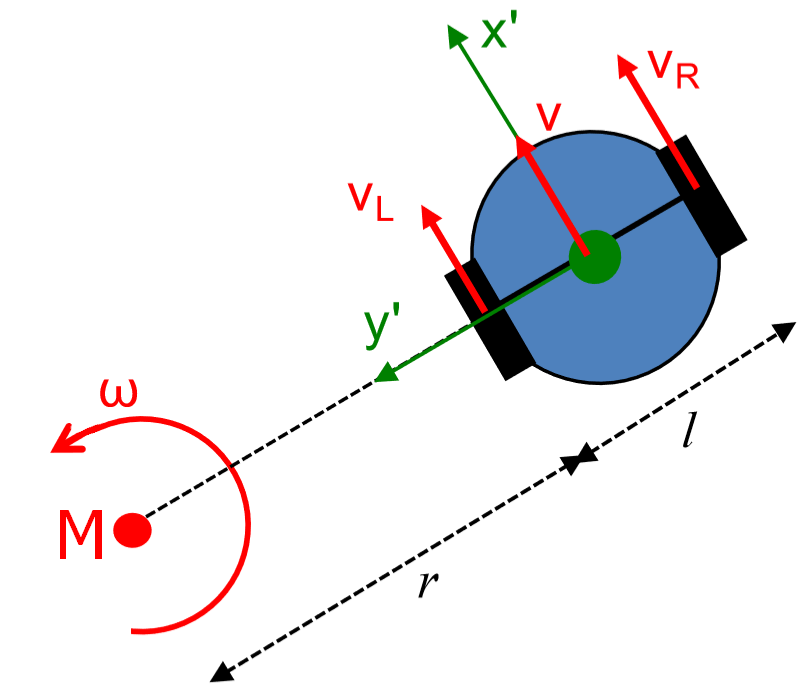
\includegraphics[scale=1]{img/einfachesModell_2.png}
  \caption{Lenkung entspricht Rotation um Momentanpol\cite{robot}}
  \label{fig:Lenkung entspricht Rotation um Momentanpol}
\end{figure}
\begin{equation}
\omega = \frac{v}{r}
\end{equation}
Der Geschwindigkeitsvektor steht dabei senkrecht zu r. Bei Ge­ra­de­aus­fahrt ist die Winkelgeschwindigkeit gleich null und r unendlich groß. \\
Kinematisches Modell: \\
Die Geschwindigkeit des linken Rades $v_{L}$ und die des rechten Rades $v_{R}$ sind voneinander unabhängig. Unser Fahrzeug bewegt sich um den Momentanpol mit Winkelgeschwindigkeit $\omega$ und Geschwindigkeit $v$ in fahrzeugfester x-Richtung.
\begin{equation}
v_{L} = \omega \cdot r
\end{equation}
\begin{equation}
v_{R} = \omega \cdot (r + l)
\end{equation}
Dabei ist $l$ die Breite des Fahrzeugs, sodass der äußerste Punkt des Fahrzeuges den Abstand $r + l$ zum Momentanpol hat. Die Räder haben die gleiche Winkelgeschwindigkeit, aber unterschiedliche Tangentengeschwindigkeiten, weil Ihr Radius sich unterscheidet. Somit hat das Fahrzeug (aufgefasst als Punkt zwischen den Rädern) die Tangentengeschwindigkeit:
\begin{equation}
v = \omega \cdot (r + \frac{l}{2})
\end{equation}
Aus $v_{L}$ und $v_{R}$ und der Achsenlänge $l$ lassen sich $v$ und $\omega$ direkt ermitteln: 
\begin{equation}
v = \frac{v_{R}+v_{L}}{2}
\end{equation}
\begin{equation}
\omega = \frac{v_{R}-v_{L}}{l}
\end{equation}
Ebenso einfach lassen sich $v_{L}$ und $v_{R}$ aus $v$ und $\omega$ bestimmen. \\
In der Realität stellt sich die gewünschte Winkelgeschwindigkeit erst mit einer gewissen Verzögerung ein, aber das lassen wir in unserem Modell unbeachtet. Analoges gilt für die Geschwindigkeit. Konkret kann man also, von den Geschwindigkeiten beider Räder ausgehend, die Geschwindigkeit und Richtung des Fahrzeugs bestimmen. Durch diese Vorgaben berechnet man, wie sich das Fahrzeug verhalten wird. Eventuelle Abweichungen von Soll-Geschwindigkeit und Soll-Richtung können gemessen und an den Regler weitergegeben werden. Dann werden die Differenzen der Soll und Ist Größen von Geschwindigkeit und Lenkwinkel errechnet. Aus den beiden Werten lassen sich dann wiederum $v_{R}$ und $v_{L}$ berechnen, die an die jeweiligen Aktuatoren weitergegeben werden.
\\
Auf einen Punkt zufahren: \\
Um unser Fahrzeug auf einen Punkt $(x_{ziel}$, $y_{ziel})$ zufahren zu lassen, muss eine Geschwindigkeit
\begin{equation}
v = K_{P} \sqrt{(x-x_{ziel})^2 + (y-y_{ziel})^2}
\end{equation}
und eine Zielrichtung 
\begin{equation}
\Theta_{ziel} = atan2(y_{ziel}-y, x_{ziel}-x)
\end{equation}
und eine Winkelgeschwindigkeit 
\begin{equation}
\omega = K_{\omega}\Delta(\theta_{ziel}, \theta)
\end{equation}
passend gewählt werden. Dabei ist $\Delta(\theta_{ziel}, \theta)$ die Winkeldifferenz aus dem Intervall $[-\pi , + \pi]$.\\
Klar ist, dass sich unser Fahrzeug nicht perfekt an die vorgegebenen Trajektorie halten kann. Ziel ist es daher, mittels Regler so nahe wie möglich der Vorgabe zu entsprechen. 
Um einer Linie zu folgen, muss der Abstand zwischen ist und soll auf null reduziert werden.
Je größer die Abweichung, desto größer die Änderung. Mittels PID-Regler wird diese Proportionalität zwischen Abstand und Winkelgeschwindigkeit erzeugt: 
\begin{equation}
\omega(t) = \underbrace{-K_{P}e(t)}_{\substack{P}} - \underbrace{-K_{I}\int {e(t)dt}}_{\substack{I}} - \underbrace{-K_{D}\frac{de(t)}{dt}}_{\substack{D}}
\end{equation}
Einstellen der Parameter $K_{P}, K_{I}, K_{D}$ mittels Faustregel (z.B. Ziegler/Nichols).














\section{Trajektorienfolgeregelung}
\label{sec:trajektorienfolgeregelung}
Zum Fahren braucht ein Fahrzeug eine Strecke, auf der es von Punkt A nach Punkt B gelangt. In unserem Modell soll sich das Fahrzeug selbst den Weg suchen, um das vorgegebene Ziel zu erreichen. In diesem Kapitel wird die autonome Berechnung einer \textit{Trajektorie} behandelt. 
Eine Trajektorie ist der geplante Sollverlauf der Fahrzeugszustandsgrößen \cite{trajDef}, beziehungsweise eine Kurve in der Ebene, parameterisiert über die Zeit. Die einzelnen Punkte der Kurve sind die Positionen zu bestimmten Zeitpunkten. Ohne die dazugehörigen Zeitinformationen, ist die Trajektorie nur ein Pfad. Dabei ist die Orientierung die Tangente des jeweiligen Punktes.
Ergebnis der Trajektorienplanung ist der zu fahrende Verlauf. Als Vorgaben erhält das Fahrzeug dafür die Koordinaten des Ziels und (gegebenenfalls) Hindernisse. 
Die aktuelle Trajektorie gibt die aktuelle Geschwindigkeit in x- und y-Richtung an.
Um aus diesen Informationen einen Pfad aussuchen zu können, der zum Ziel führt, muss es ein Bewertungsschema geben. Es gibt unendlich viele Wege, aus denen das Fahrzeug wählen kann, aber nur einen kürzesten. Das Kriterium für einen guten Pfad ist also äquivalent zu seiner Länge. Ohne Hindernisse ist das einfach eine Gerade vom Ausgangspunkt zum Ziel, und das Fahrzeug kann ohne Regelung die Aufgabe erledigen.
Mithilfe von Matlab lässt sich eine Simulation entwickeln, die den Pfad zwischen Start und Ziel auf einem zweidimensionalen Koordinatensystem zeigt \cite{ml}. 
\lstset{language=Matlab}          
\begin{lstlisting}[frame=single]
%% EXAMPLE: Differential Drive continuous simulation
R = 0.1;                % Wheel radius [m]
L = 0.5;                % Wheelbase [m]
dd = DifferentialDrive(R,L);

%% Run a continuous simulation using ODE45
initPose = [0 0 pi/4];  % Initial pose (x y theta)
tspan = [0 10];
[t,pose] = ode45(@(t,y)diffDriveDynamics(t,y,dd),tspan,initPose);
pose = pose';

%% Display results
close all
figure
hold on
plot(pose(1,1),pose(2,1),'ro', ...
     pose(1,end),pose(2,end),'go', ...
     pose(1,:),pose(2,:),'b-');
axis equal
title('Vehicle Trajectory');
xlabel('X [m]')
ylabel('Y [m]')
legend('Start','End','Trajectory')


%% Continuous dynamics
function dy = diffDriveDynamics(t,y,vehicle)
    
    % Set desired velocities and solve inverse kinematics
    vDes = 0.2;
    if t < 5
       wDes = -0.5; 
    else
       wDes = 0.5;
    end
    [wL,wR] = vehicle.inverseKinematics(vDes,wDes);
    
    % Calculate forward kinematics and convert the speeds to global
    [v,w] = vehicle.forwardKinematics(wL,wR);
    velB = [v;0;w];            % Body velocities [vx;vy;w]
    dy = bodyToWorld(velB,y);  % Convert from body to world
end
\end{lstlisting}
Durch Ausführung dieses Codebeispiels in Matlab wird das in Abbildung 3.3 gezeigte Bild erzeugt. 
\begin{figure}[htb] 
  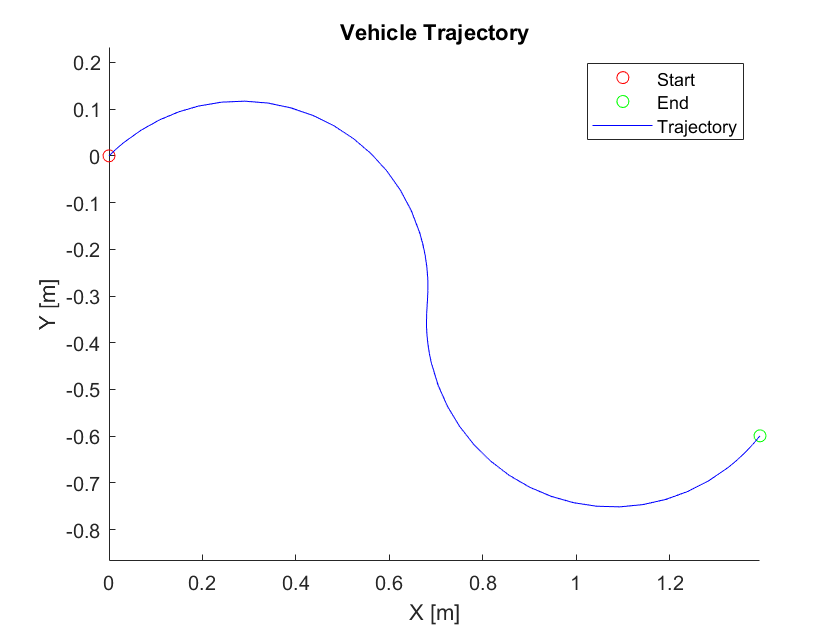
\includegraphics[scale=0.8]{img/einacherPfad.png}
  \caption{MATLAB Beispiel}
  \label{fig:MATLAB Beispiel}
\end{figure}
Bei diesem Modell wird der 'pure pursuit path tracking' (pure Verfolgung) Algorithmus verwendet, um nacheinander die auf einem Weltfestem Koordinatensystem vorhandenen Wegpunkte abzufahren. Bei der puren Verfolgung handelt es sich um eine bewährte Methode, die sich bildhaft mittels Karotte und Esel veranschaulichen lässt. Eine Karotte ist in einem festen Abstand zum Esel an dem Esel befestigt. Der Esel sieht die Karotte vor sich und während er ihr sich vermeintlich nähert, bewegt sie sich mit der gleichen Geschwindigkeit, von ihm weg. Bei der puren Verfolgung bewegt sich ein Zielpunkt über die gewünschte Strecke, die in diesem Fall einfach eine Gerade zwischen Fahrzeug und Ziel ist. Der PID-Regler sorgt dafür, dass das Fahrzeug einen konstanten Abstand zum dynamischen Zielpunkt beibehält. Das Fahrzeug jagt also einem auf dem Pfad entlang verlaufenden Punkt hinterher. Ein weiterer Regler ist für die Ausrichtung des Fahrzeugs in dynamische Zielrichtung verantwortlich. Das bedeutet, dass das Fahrzeug nur genau dann schneller als das dynamische Ziel ist, wenn die Ausrichtung nicht zum Ziel ist. \\
Bei passend gewählter Geschwindigkeit, Winkelgeschwindigkeit und Abstand zum dynamischen Zielpunkt, nähert sich der Ausrichtungswinkel in immer kleiner werdenden Anpassungen, dem Pfad an, ohne ihn zu überschreiten und wieder zurück lenken zu müssen. Dafür müssen die Geschwindigkeiten antiproportional zum Abstand zum dynamischen Ziel sein. \\
Kurz gefasst kann man die Pure Verfolgung in folgenden Schritten skizzieren, die ständig der Reihe nach abgearbeitet werden:
\begin{itemize}
\item aktuelle Pose des Fahrzeugs bestimmen
\item den dynamischen Zielpunkt finden
\item die Zielpunktkoordinaten in Fahrzeugkorrdianten transformieren
\item das Fahrzeug darauf zufahren lassen [Link zur Textstelle in der Modellierung in der das genauer erleutert wird]
\end{itemize} 
\begin{figure}[htb]
  \centering  
  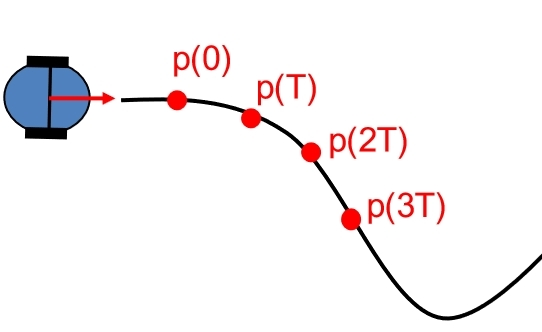
\includegraphics[scale=1.4]{img/purePursuit.jpg}
  \caption{Pure Pursuit Veranschaulichung\cite{robot}}
  \label{fig:starwars}
\end{figure}
Dieses Kapitel war geprägt von mathematischer Modellierung und Herleitung gesuchter Gleichungen aus der Physik. Als Resultat konnte ein Fahrzeugmodell entwickelt werden, das sich anhand von Eingabeparametern, auf Längs- und Querdynamik simulieren lässt, wie im nächsten Kapitel vorgemacht.\\